\definecolor{greenish}{RGB}{0,145,0}
\begin{tikzpicture}
	\pgfplotsset{/tikz/font={\small}}
	\begin{axis}[
			% title=Bitrate savings: $-8.94\%$. SNR improvement: $0.46$ dB,
			xlabel={ROM (kB)},
			ylabel={Y BD-rate (\%)},
			grid=both,
			scale only axis,
			width=0.9\textwidth,
			height=0.3\textheight,
			xtick={0.25,0.5,1,2,4,8,16,32,64,128,256,512,1024},
			xticklabels={0.25,0.5,1,2,4,8,16,32,64,128,256,512,1024},
			% x tick label style={
			% 	/pgf/number format/.cd,
			% 	fixed,
			% 	fixed zerofill,
			% 	precision=0,
			% },
			% scaled x ticks=false,
			ytick={0,-0.5,...,-4},
			y tick label style={
				/pgf/number format/.cd,
				fixed,
				fixed zerofill,
				precision=1,
				/tikz/.cd
			},
			xmode=log,
			log basis x=2,
			xmin=0.5, xmax=256,
			ymin=-4.0, ymax=0,
			legend style={nodes=right},
			legend pos= south west
		]

		\addlegendentry{Comb.\ non-hom.\ non-sym. MDTC}
		\addplot [mark=*, mark size=1pt, blue, thick,
		visualization depends on=\thisrow{alignment} \as \alignment,
		nodes near coords, % Place nodes near each coordinate
		point meta=explicit symbolic, % The meta data used in the nodes is not explicitly provided and not numeric
		every node near coord/.style={anchor=\alignment} % Align each coordinate at the anchor 40 degrees clockwise from the right edge
		] table [meta index=2] {
		rom	bdrate	label	alignment
		0.98	-0.74 \tiny{\color{black}1 kB}	270
		1.97	-1.02 \tiny{\color{black}2 kB}	270
		3.98	-1.39 \tiny{\color{black}4 kB}	270
		7.97	-1.82 \tiny{\color{black}8 kB}	270
		12.00	-2.10 \tiny{\color{black}12 kB}	0
		15.61	-2.22 \tiny{\color{black}16 kB}	0
		23.95	-2.52 \tiny{\color{black}24 kB}	0
		31.78	-2.68 \tiny{\color{black}32 kB}	0
		47.39	-2.85 \tiny{\color{black}48 kB}	0
		63.89	-3.00 \tiny{\color{black}64 kB}	0
		95.53	-3.27 \tiny{\color{black}96 kB}	0
		127.41	-3.41 \tiny{\color{black}128 kB}	0
		};

		\addlegendentry{Comb.\ non-hom.\ sym. MDTC}
		\addplot [mark=*, mark size=1pt, greenish, thick,
		visualization depends on=\thisrow{alignment} \as \alignment,
		nodes near coords, % Place nodes near each coordinate
		point meta=explicit symbolic, % The meta data used in the nodes is not explicitly provided and not numeric
		every node near coord/.style={anchor=\alignment} % Align each coordinate at the anchor 40 degrees clockwise from the right edge
		] table [meta index=2] {
		rom	bdrate	label	alignment
		0.98	-0.89 \tiny{\color{black}1 kB}	0
		1.92	-1.25 \tiny{\color{black}2 kB}	0
		3.98	-1.71 \tiny{\color{black}4 kB}	-135
		7.88	-2.16 \tiny{\color{black}8 kB}	0
		11.62	-2.39 \tiny{\color{black}12 kB}	0
		15.84	-2.51 \tiny{\color{black}16 kB}	0
		23.67	-2.83 \tiny{\color{black}24 kB}	0
		31.92	-2.97 \tiny{\color{black}32 kB}	0
		48.00	-3.13 \tiny{\color{black}48 kB}	0
		63.80	-3.28 \tiny{\color{black}64 kB}	0
		88.90	-3.45 \tiny{\color{black}96 kB}	0
		123.40	-3.56 \tiny{\color{black}128 kB}	0
		};

		\addlegendentry{Comb.\ non-hom.\ sym DTT-MDTC}
		\addplot [mark=*, mark size=1pt, red, thick,
		visualization depends on=\thisrow{alignment} \as \alignment,
		nodes near coords, % Place nodes near each coordinate
		point meta=explicit symbolic, % The meta data used in the nodes is not explicitly provided and not numeric
		every node near coord/.style={anchor=\alignment} % Align each coordinate at the anchor 40 degrees clockwise from the right edge
		] table [meta index=2] {
		rom	bdrate	label	alignment
		0.98	-1.28 \tiny{\color{black}1 kB}	0
		1.97	-1.54 \tiny{\color{black}2 kB}	15
		3.97	-1.83 \tiny{\color{black}4 kB}	15
		};

\end{axis}
\end{tikzpicture}
